\subsection{Data Sets}

\label{sec:data_sets}

Experimental evaluations are conducted on three data sets: Halo 2 XBox Live
matches, Australian Football
(Rugby) League (AFL)%\footnote{\noindent
%  \url{http://www.csse.monash.edu.au/~footy/data/index.shtml}}
and UK
Premier League (UK-PL)\footnote{\noindent \url{http://www.football-data.co.uk/englandm.php}}.  The Halo 2 data consists of a
set of match outcomes comprising 6227 games for 1672 players. We note there are negative scores for this data, so we add the absolute value of the minimal score to all scores to use the data with all proposed models.

The training and testing settings are described as follows.  For Halo
2~\footnote{\noindent Credit for the use of the Halo 2 Beta Data set
is given to Microsoft Research Ltd. and Bungie.}, the last 10\%
of matches are used for testing, and we use different proportions of
the first 90\% of data for training. There are 8 proportions used
for training, ranging from 10\% to 80\% with an increment of
10\%, and 90\% is not used for training due to cross validation. To cross validate, we sample the data and run the learning 20 times at each proportion level
to get standard error bars. Note that there are some players in the
testing games who are not involved in any training data sets,
particularly when small proportion of training data set is selected
(e.g., the first 10 percent games); we remove these games in the
testing set when reporting performances for all models.

For both UK-PL and AFL datasets, cross validation is performed by
training and testing for each year separately (14 years for UK-PL, and
11 years for AFL).  For these two datasets, we test the last 20\%
percent of matches in each year, with the training data increasing
incrementally from 10\% to 80\% of the initial matches.

\subsection{Evaluation Criteria}

We evaluate performances using three criteria: {\it information gain}
of predicting winning probability of a team
(Section~\ref{sec:informationGain}),
{\it win/lose prediction accuracy}
(Section~\ref{sec:WLPredictionAccuracy}),
and {\it score prediction errors}
(Section~\ref{sec:scorePredictionError}).
While the first two criteria focus on predicting win/lose, the third
criterion measures how good a model is at predicting scores, for which
TrueSkill does not apply since it is restricted to WLD only. Let us
introduce each criterion in detail.

\subsubsection{Information Gain}
\label{sec:informationGain}

The first criterion we use to evaluate different approaches is
\emph{information gain}, which is proposed in the \emph{Probabilistic Footy
Tipping Competition}\footnote{Refer to
\url{http://www.csse.monash.edu.au/~footy/}}: if a predictor assigns
probability $p$ to team $i$ winning, then the score (in ``bits")
gained is $1+\log_2(p)$ if team $i$ wins, $1+\log_2(1-p)$ if team $i$ loses, $1+(1/2)\log_2(p(1-p))$ if draw happens.
This evaluation metric can be viewed as an information gain
interpretable variant of a log likelihood score where an uninformed
prediction of $p=0.5$ leads to a score of 0 and a definite prediction
of $p=1$ ($p=0$) leads to a score of $-\infty$ if predicting
incorrectly and 1 if predicting correctly.
In Section~\ref{sec:inference}, we showed how to compute the win
probability $p$ for each model.

\subsubsection{Win/no-Win Prediction Accuracy}
\label{sec:WLPredictionAccuracy}

While information gain provides a sense of how well the models fit the
data, it is also interesting to see how accurate the models were at
predicting match outcomes in terms of win/no-win (e.g., loss/draw).  To compare
classification performance of each model, we report the
win/not winning prediction accuracy in terms of area under the curve (AUC) for the
games with a win or loss outcome.

%This is a straighforward metric to
%evaluate in expectation: for the univariate skill models we simply
%assign a win to the team with the higher mean skill level, for the
%remaining offence/defence score models, we simply assign a win to the
%team with the higher expected score (these simple calculations are
%explained in the next subsection).

%It is essential to evaluate the prediction accuracy in terms of
%win/loss for matchmaking. To describe this evaluation criterion, let
%us first introduce when a model predicts team $i$ winning, in a match
%with team $j$. Based on the belief of a model, its prediction is
%correct: either (1) team $i$'s mean skill is larger than that of team
%$j$ skill and team $i$ wins, or (2) team $i$'s mean skill is smaller
%than that of team $j$ skill and team $i$ loses. Suppose there are $M$
%matches, and the model predicts correctly for $N$ times, then the
%prediction accuracy is $N/M$.

\subsubsection{Score Prediction Error}
\label{sec:scorePredictionError}

%We evaluate the score prediction accuracy for the two full
% score prediction models: Poisson-OD and Gaussian-OD.
%For the Poisson-OD model (Figure~\ref{fig:trueskill_variant}), the
%expected score for team $i$ ($j$) is $\exp(x)$ ($\exp(y)$) and for the
%Gaussian-OD model
%(Figure~\ref{fig:modelAndInferenceGaussianGraphicalModel}), the
%expected score for team $i$ ($j$) is $x$ ($y$), where $x$ ($y$) is the
%difference in mean performances giving $s_i$ ($s_j$).  The Gaussian-SD model
%(Figure~\ref{fig:modelAndInferenceGaussianGraphicalModelScoreDifference}),
%directly produces \emph{score difference} predictions $d = s_i - s_j$,
%which is just the difference in mean performances of the two teams.
%Because scores for different games have a different scale, we introduce
%a relative measure of score accuracy.
%Suppose $s^*$ is the true score, and
%$\hat{s}$ the expected score. We define the
%relative score prediction error $e(s^*, \hat{s})$ as
%\begin{align}
%e(s^*, \hat{s})= \frac{|\hat{s}-s^*|}{|s^*|}.
%\end{align}
%%Therefore, the larger the deviation of $\hat{s}$ to the true score $s^*$, the larger the error.
%Note that the prediction error can be larger than one,
%e.g. $\hat{s}=5, s^*=2$ causing $e(s^*, \hat{s})=1.5$.




%For the Poisson-OD model (Figure~\ref{fig:trueskill_variant}), the
%expected score for team $i$ ($j$) is $\exp(x)$ ($\exp(y)$) and for the
%Gaussian-OD model
%(Figure~\ref{fig:modelAndInferenceGaussianGraphicalModel}), the
%expected score for team $i$ ($j$) is $x$ ($y$), where $x$ ($y$) is the
%difference in mean performances giving $s_i$ ($s_j$).  The Gaussian-SD model
%(Figure~\ref{fig:modelAndInferenceGaussianGraphicalModelScoreDifference}),
%directly produces \emph{score difference} predictions $d = s_i - s_j$,
%which is just the difference in mean performances of the two teams.
We evaluate the score prediction accuracy for Poisson-OD and
Gaussian-OD models for \emph{each} team in terms of the mean absolute
error (MAE). Note that we must omit the Gaussian-SD model since it can only
predict score differences rather than scores.

%, defined as below:
%{\small\begin{align}
%    \text{MAE} = \frac{1}{n} \sum_{i=1}^{2*n} | \hat{s_i} - s_i |
%\end{align}}
%where $\hat{s_i}$ is the predicted score, $s_i$ the ground truth, and $n$ the number of matches for matches involving two players.

%The MAE for the Gaussian-SD model is given as below.
%\begin{align}
%    \text{MAE} = \frac{1}{n} \sum_{i=1}^{n} | \hat{\text{sd}_i} - \text{sd}_i |
%\end{align}
%where $\hat{\text{sd}_i}$ is the predicted score difference for match $i$, and $\text{sd}_i$ is the ground truth for the score difference of match $i$.

% \subsection{Logistic Regression}
% Perhaps the simplest score prediction approach is to use a linear regression model for $m$ teams and $n$ matches with variables $o_1,\ldots,o_m$ and $d_1,\ldots,d_m$
% can be setup as in the following example:
% \begin{equation*}
%     \underbrace{\begin{pmatrix}
%         1 & 0 & 0 & -1 & \dots & 0 & 0 \\
%         0 & -1 & 1 & 0 & \dots & 0 & 0 \\
%         0 & -1  & 0 & 0 & \dots & 1 & 0 \\
%         1 & 0  & 0 & 0 & \dots & 0 & -1 \\
%         \hdotsfor{7}                   \\
%         0 & 0  & 1 & 0 & \dots & 0 & -1\\
%         0 & 0  & 0 & -1 & \dots& 1 & 0
%     \end{pmatrix}}_{A}
%     \underbrace{\begin{pmatrix}
%         o_1 \\
%         d_1 \\
%         o_2 \\
%         d_2 \\
%         \hdotsfor{1} \\
%         o_m \\
%         d_m
%     \end{pmatrix}}_{\vec{z}}
%     =
%     \underbrace{\begin{pmatrix}
%         s_{1,1} \\
%         s_{1,2} \\
%         s_{2,m} \\
%         s_{2,1} \\
%         \hdotsfor{1} \\
%         s_{n,2} \\
%         s_{n,m}
%     \end{pmatrix}}_{\vec{s}},
% \end{equation*}
% where $s_{k,j},k=1,\dots,n$ is the team $j$'s score for the $k$th match. In order to use a logistic model, we propose mapping from $s_{kj},k=\{1,\dots,n\}$ to $t_{jk}$ by
% \begin{align*}
%     t_{jk} = \frac{1}{1+\exp(-s_{jk})}.
% \end{align*}
% Now the objective is to find the optimal skill vector $z^*$ defined as
% \begin{align*}
%     z^* = \arg\min_{z}||Az-\vec{t}||_{2}^2,
% \end{align*}
% which can be achieved by using maximum likelihood parameter estimation.


\subsection{Results}

\label{sec:results}

Experimental results are reported according to the parameter
configurations shown in Table~\ref{table:Parameters}. All results are
presented in Figure~\ref{fig:Results} and discussed below.
%\begin{table}
%\vspace{-5mm}
%\caption{Parameter settings. Priors on offence/defence skills: $\mathcal{N}(\mu_{0},\sigma_{0}^2)$ with $\mu_{0}=25$ and $\sigma_{0}=25/3$. Performance variance: $\beta$, $\beta_1$, $\beta_2$.}
%\begin{center}
%\small
%\begin{tabular}{|c|c|}
%  \hline
%  Model             & Parameter ($\epsilon,\gamma$ empirically estimated)\\
%  \hline
%  TrueSkill          & $\beta=\sigma_{0}/2$; \\
%                          & $\epsilon$: draw probability of datasets\\
%\hline
%  Poisson-OD         & $\beta_1=\beta_2=\sigma_{0}/2$\\
%\hline
%  Gaussian-OD    & $\beta_1=\beta_2=\sigma_{0}/2$;\\
%                         & $\gamma$: score variance in datasets\\
%\hline
%  Gaussian-SD & $\beta=\sigma_{0}/2$;  \\
%                        & $\gamma$: score difference variance in datasets\\
%  \hline
%\end{tabular}
%\label{table:Parameters}
%\end{center}
%\vspace{-5mm}
%\end{table}
{\small\begin{table}[htbp!]
\caption{Parameter settings. Priors on offence/defence skills: $\mathcal{N}(\mu_{0},\sigma_{0}^2)$ with $\mu_{0}=25$ and $\sigma_{0}=25/3$. Performance variance: $\beta$, $\beta_o$, $\beta_d$.}
\begin{center}
\small
\begin{tabular}{cc}
  \hline
  Model             & Parameter ($\epsilon,\gamma$ empirically estimated)\\
  \hline
  TrueSkill          & $\beta=\sigma_{0}/2$, $\epsilon$: draw probability\\
  Poisson-OD         & $\beta_o=\beta_d=\sigma_{0}/2$\\
  Gaussian-OD    & $\beta_o=\beta_d=\sigma_{0}/2$, $\gamma$: score variance\\
  Gaussian-SD & $\beta=\sigma_{0}/2$, $\gamma$: score difference variance\\
  \hline
\end{tabular}
\label{table:Parameters}
\end{center}
\end{table}}

%%%%%%%%%%%%%%%%%%%%%%%%%%%%%%%%%%%%%%%%%%%%%%%%%%%%%%%%%%%%%%%%%
\begin{center}
\begin{figure*}[t!]
 \centering
 \subfigure{
   \hspace{-1.2cm}
   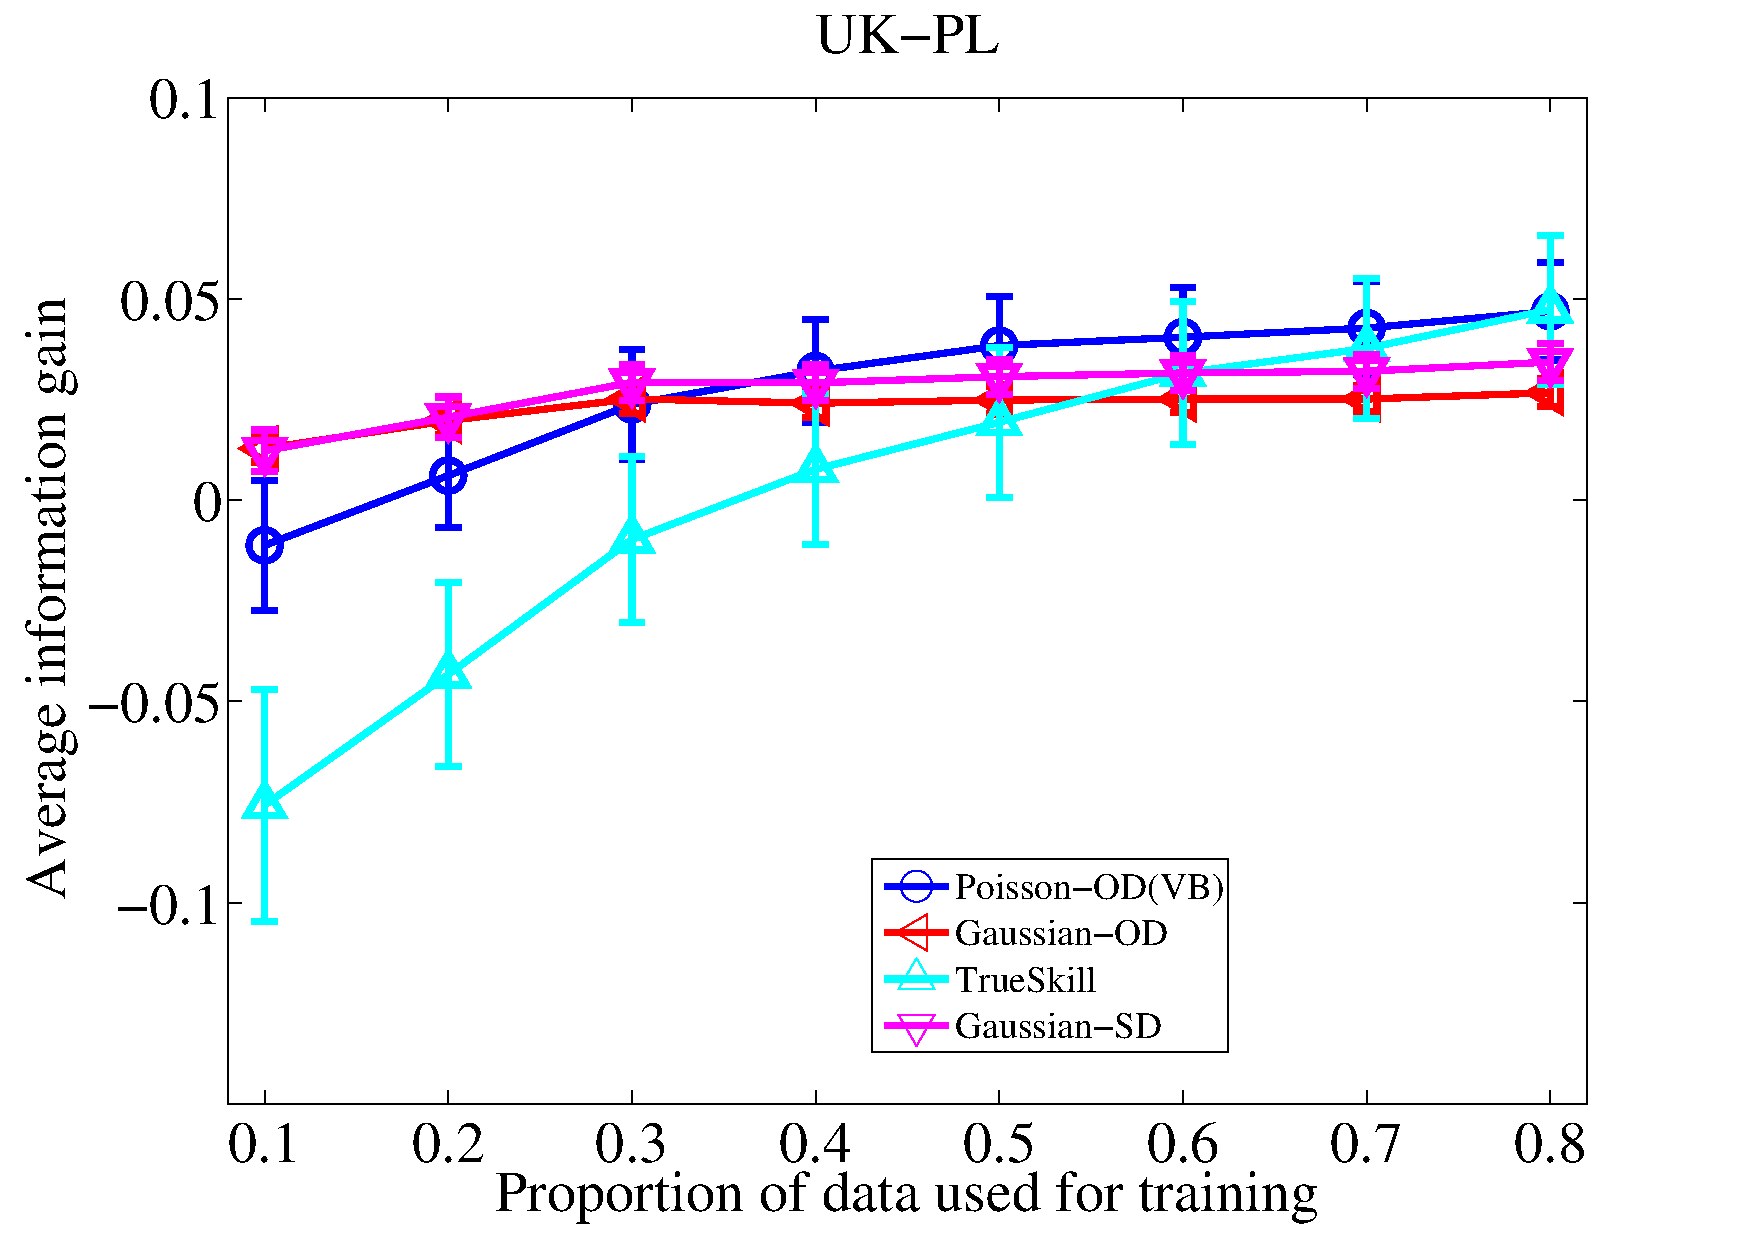
\epsfig{file=InforGain_UK, angle=0, height=3.6cm}
   \hspace{-0.725cm}
   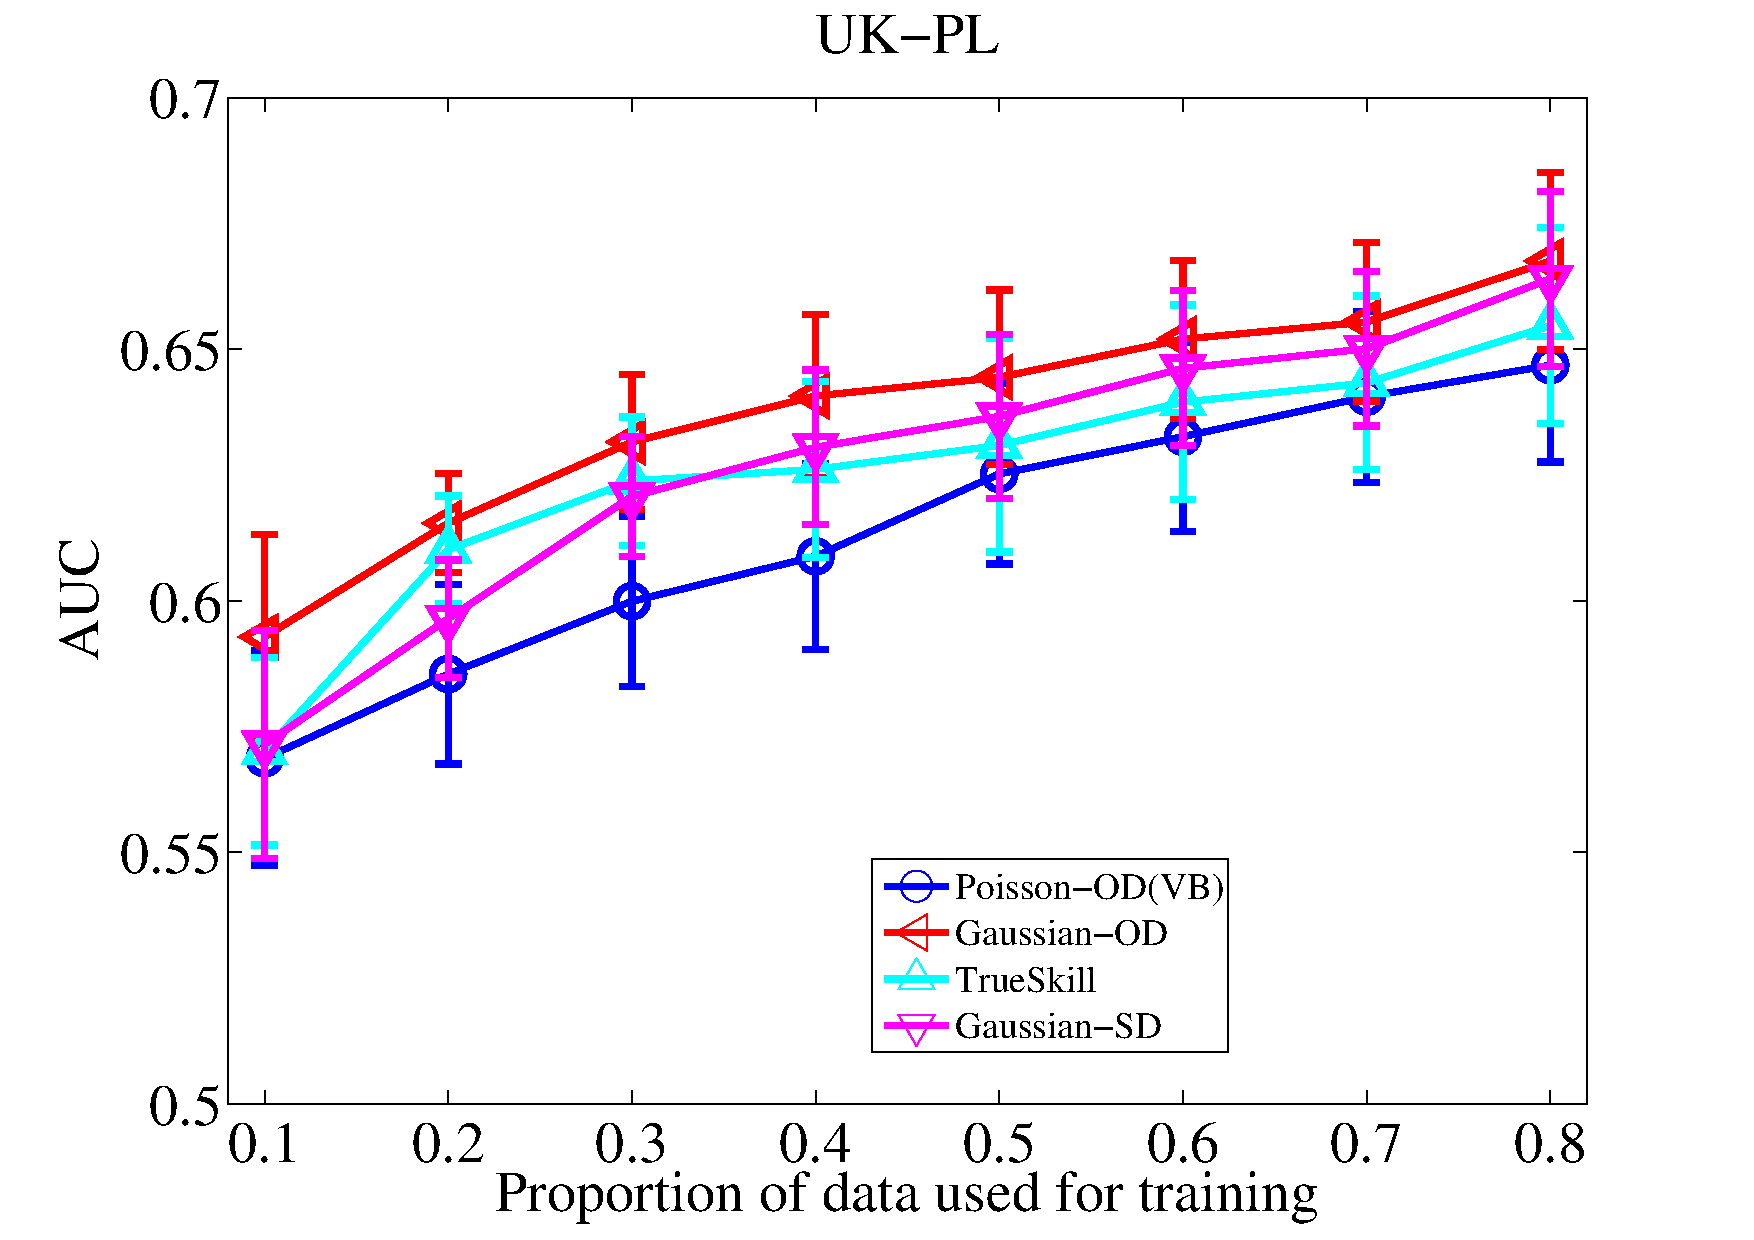
\epsfig{file=WLAccuracy_UK, angle=0, height=3.6cm}
   \hspace{-0.725cm}
   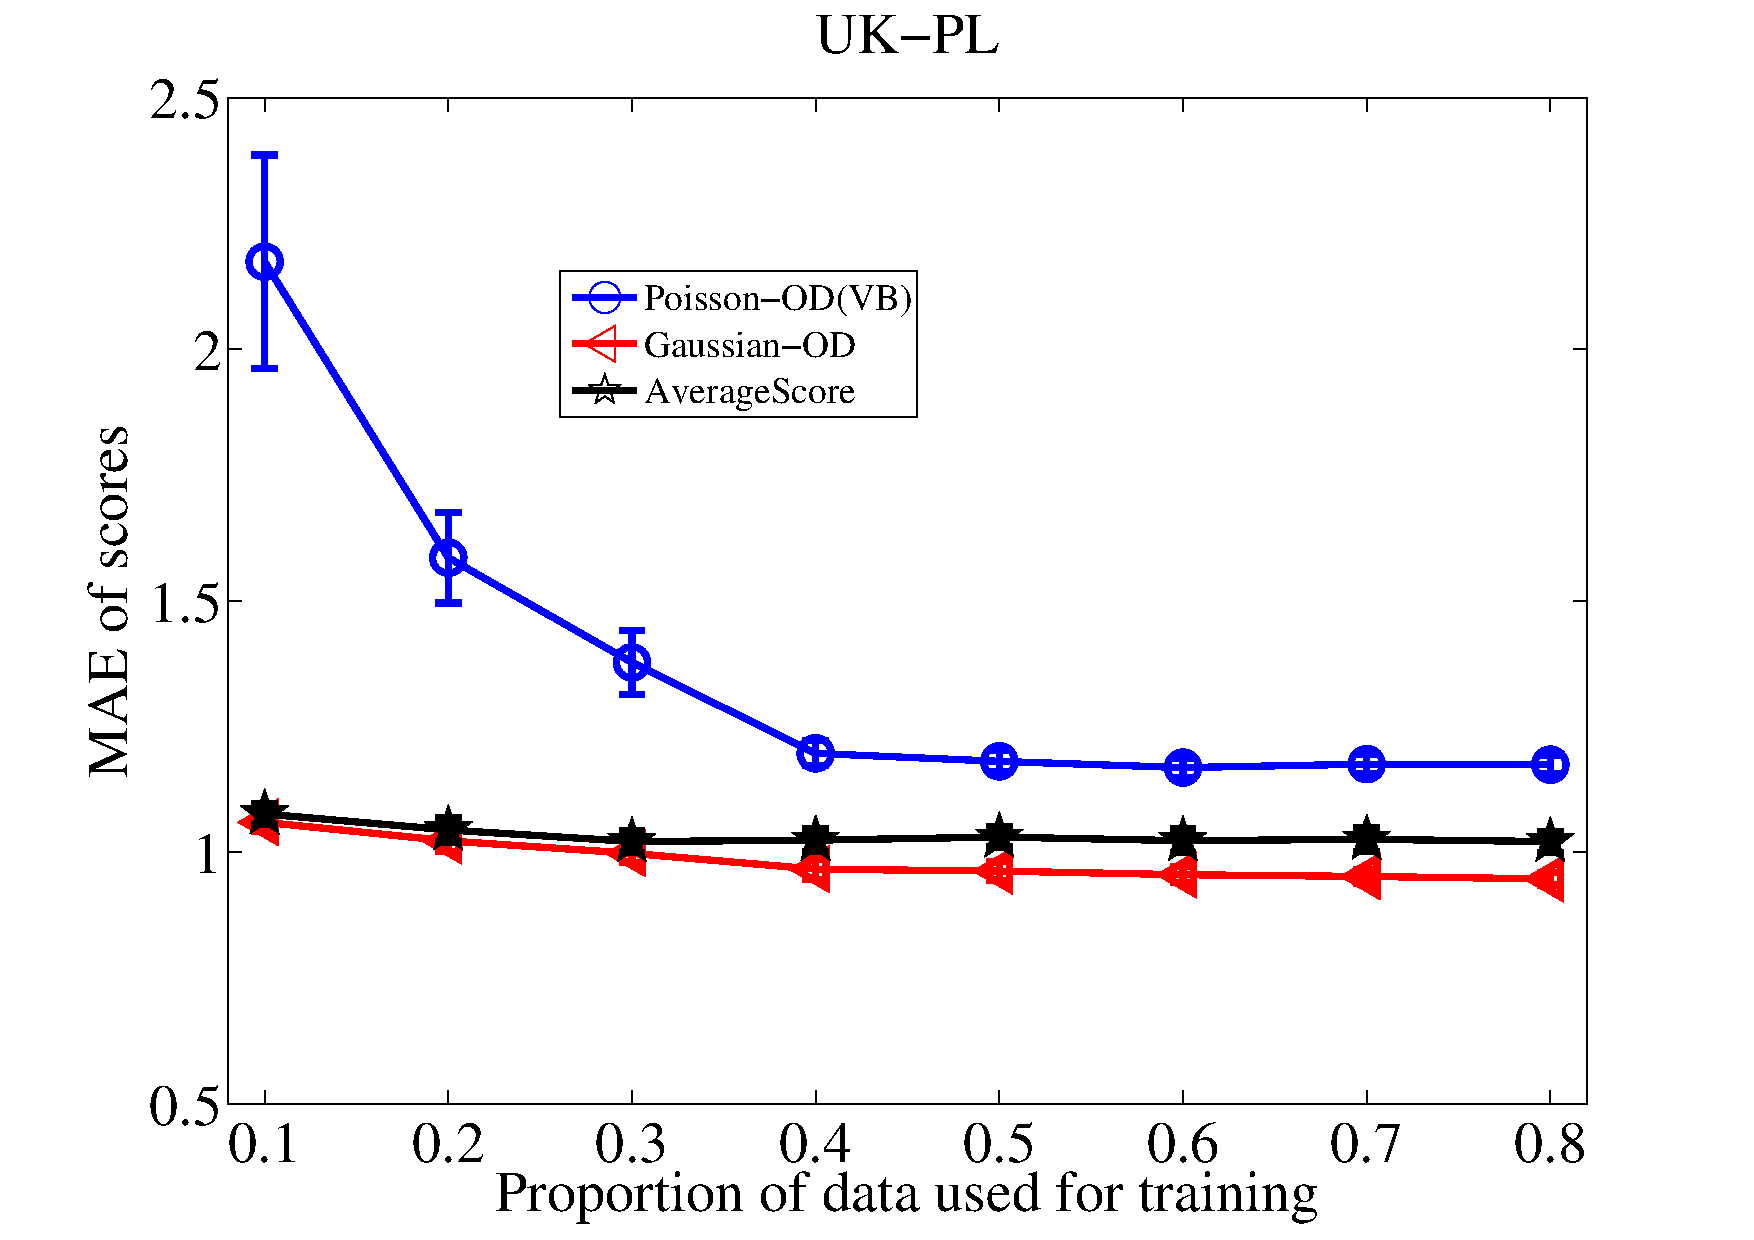
\epsfig{file=ScoreError_UK, angle=0, height=3.6cm}
 }\\
 \subfigure{
    \hspace{-1.2cm}
   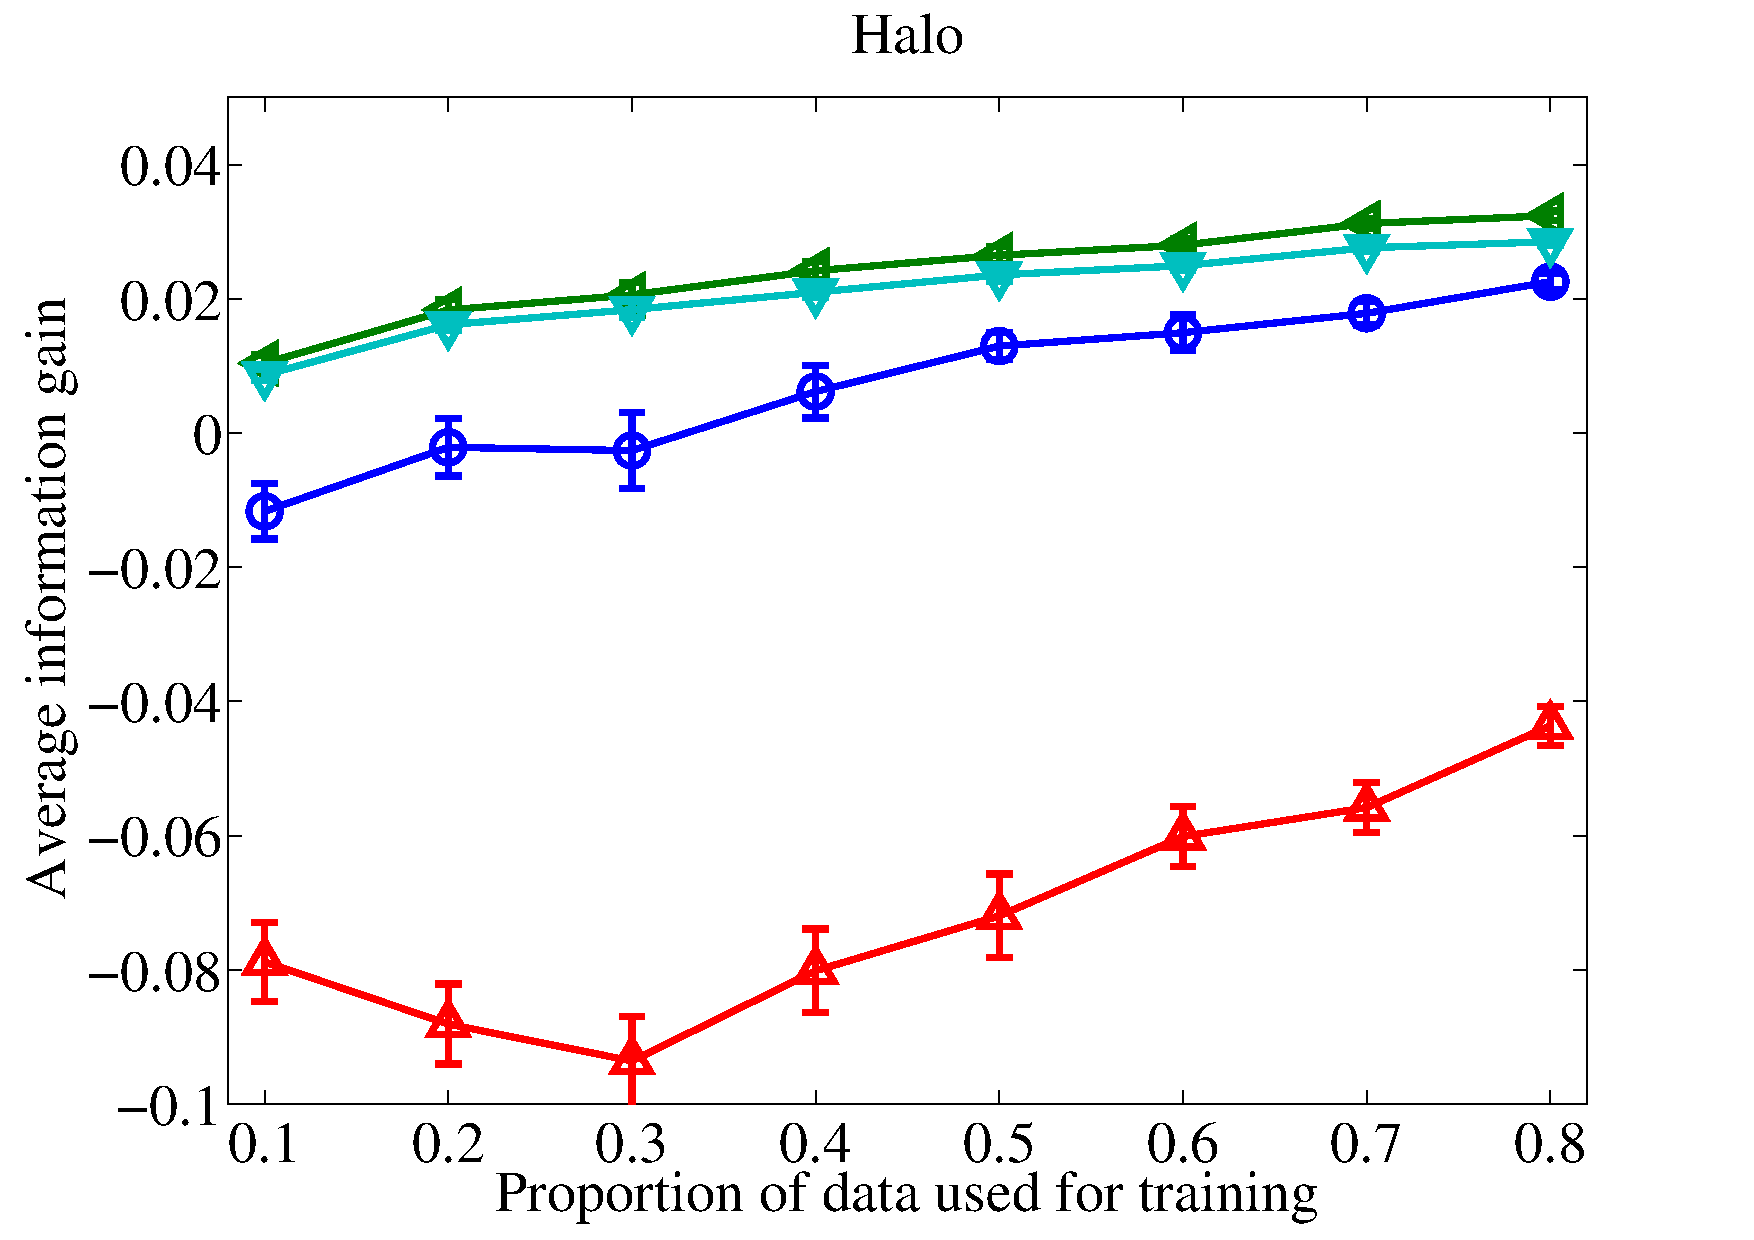
\epsfig{file=InforGain_Halo, angle=0, height=3.6cm}
   \hspace{-0.725cm}
   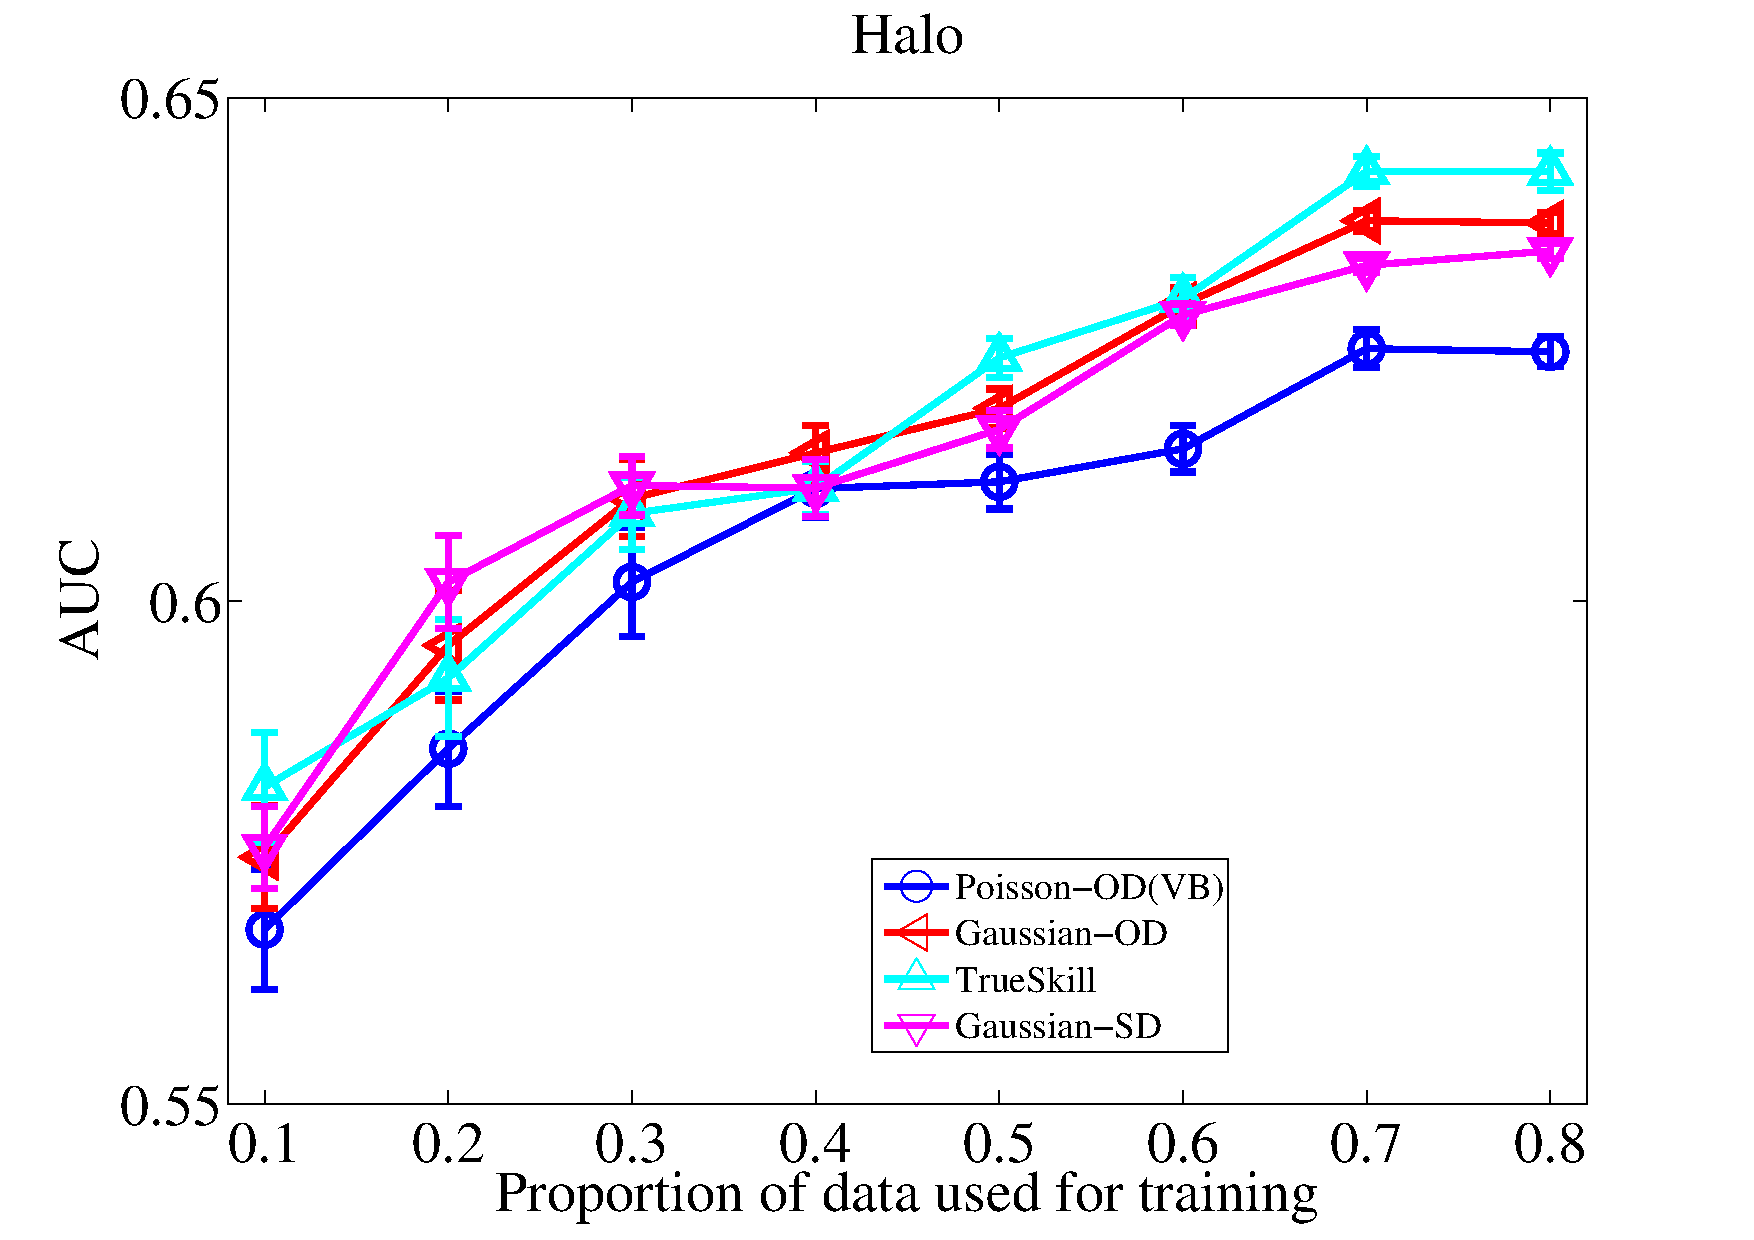
\epsfig{file=WLAccuracy_Halo, angle=0, height=3.6cm}
   \hspace{-0.725cm}
   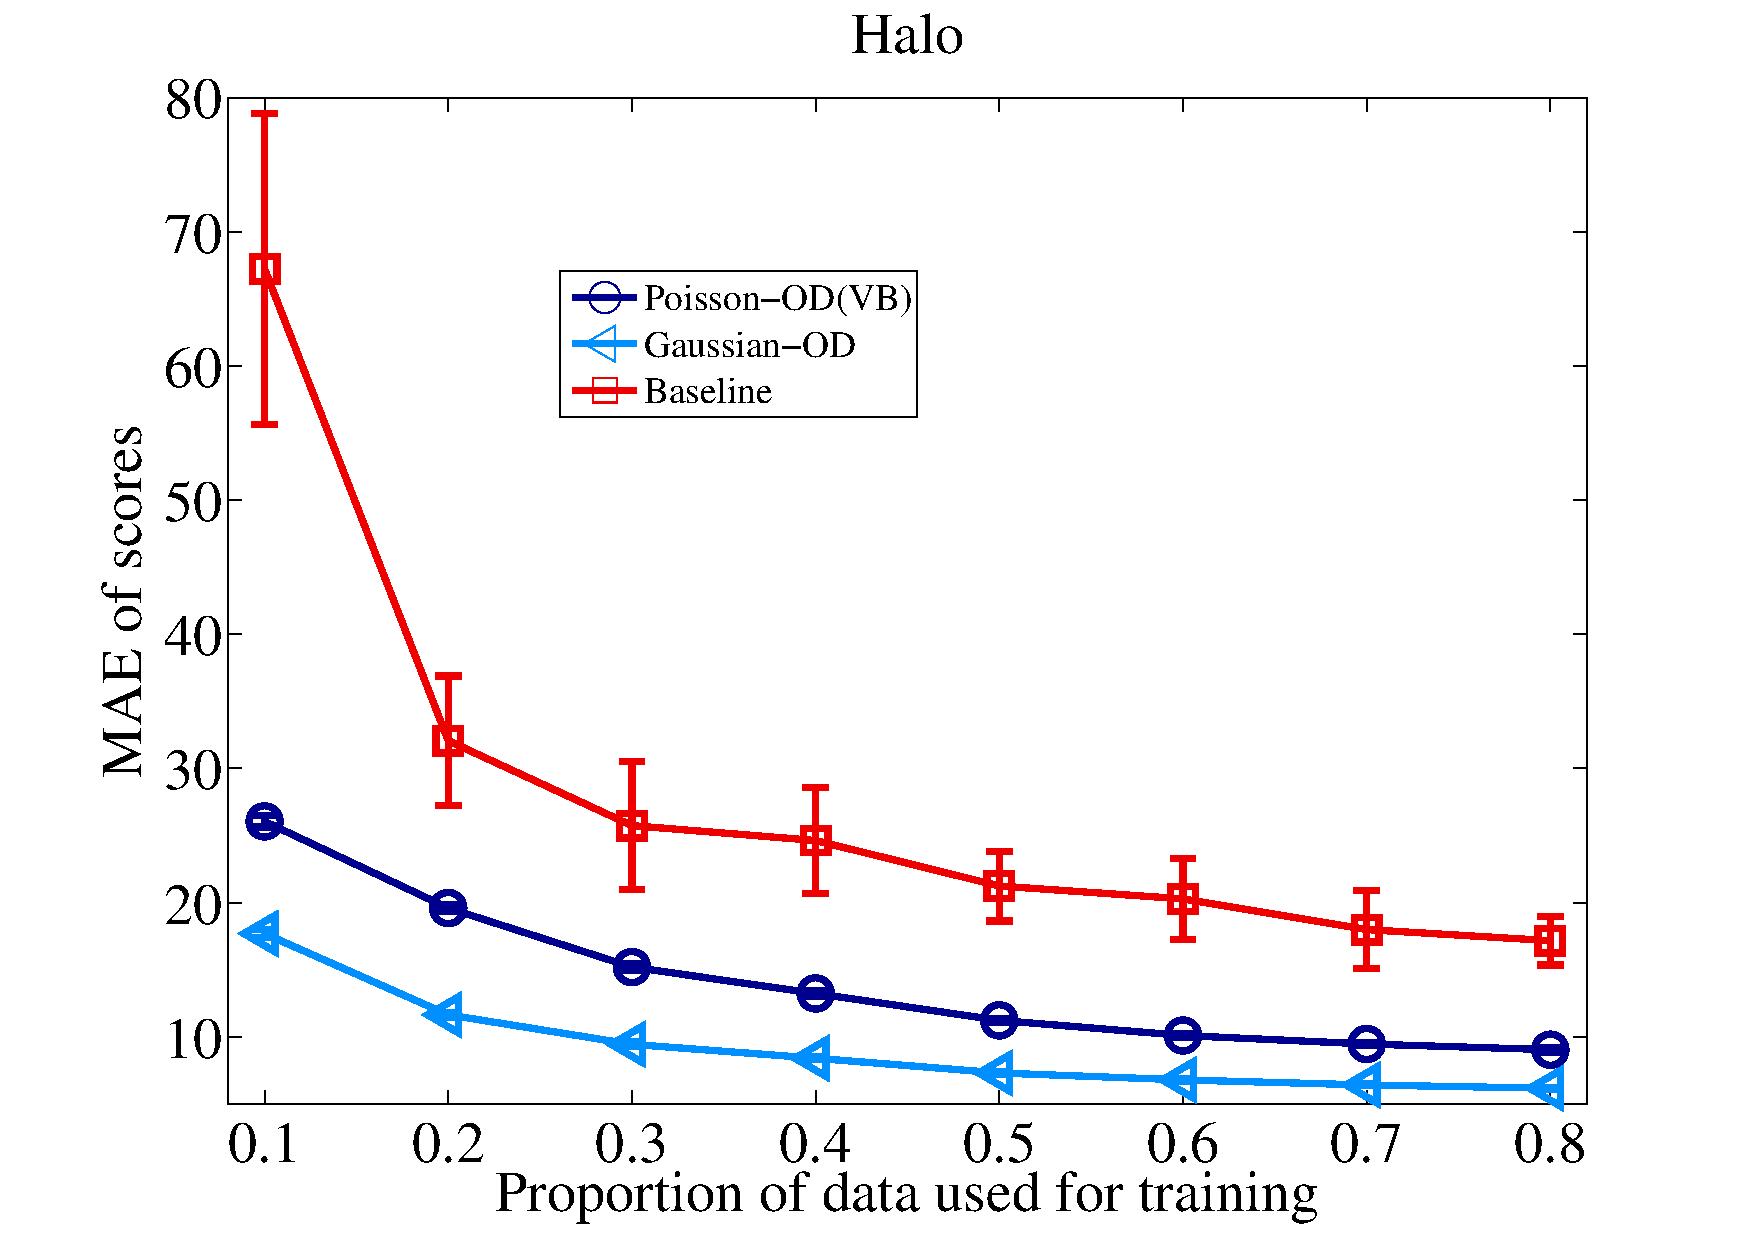
\epsfig{file=ScoreError_Halo, angle=0, height=3.6cm}
 }\\
 \subfigure{
    \hspace{-1.2cm}
   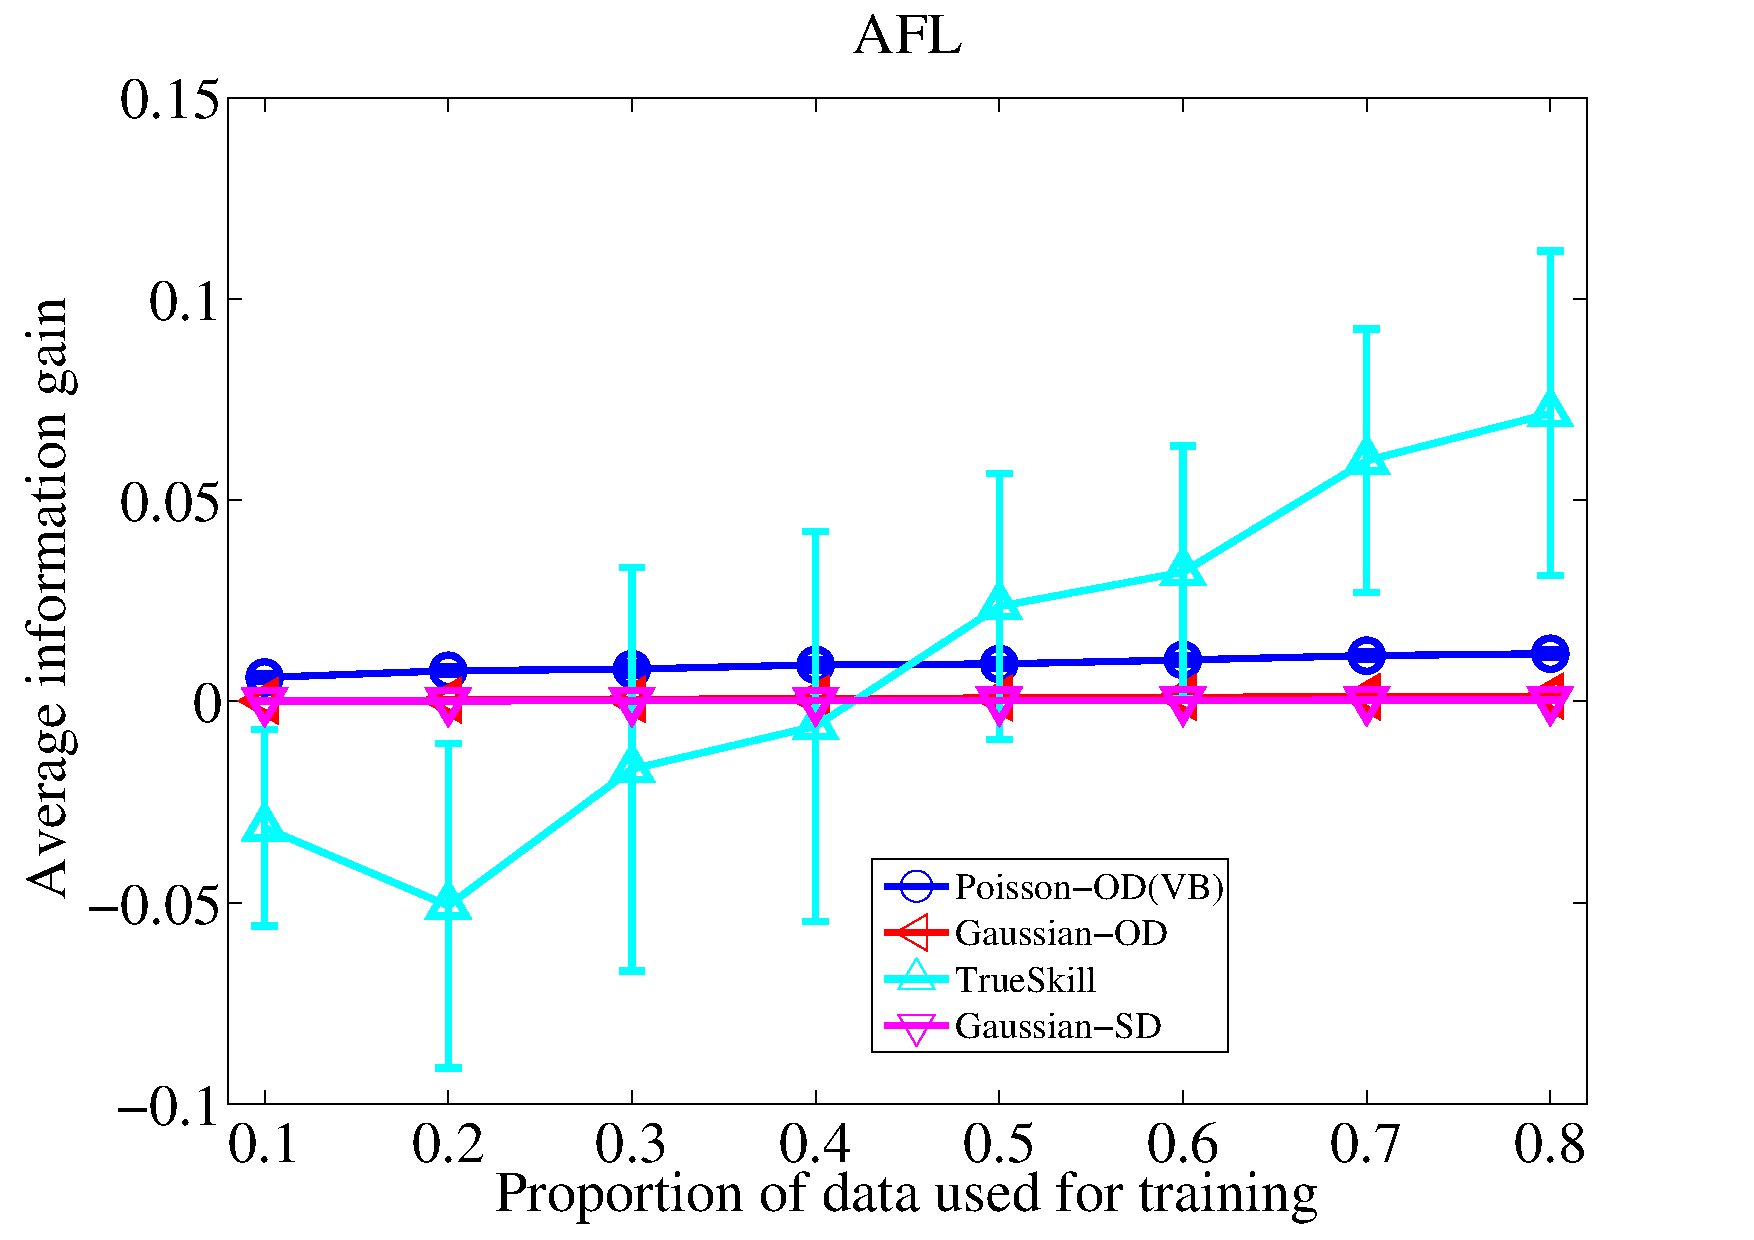
\epsfig{file=InforGain_AFL, angle=0, height=3.6cm}
   \hspace{-0.725cm}
   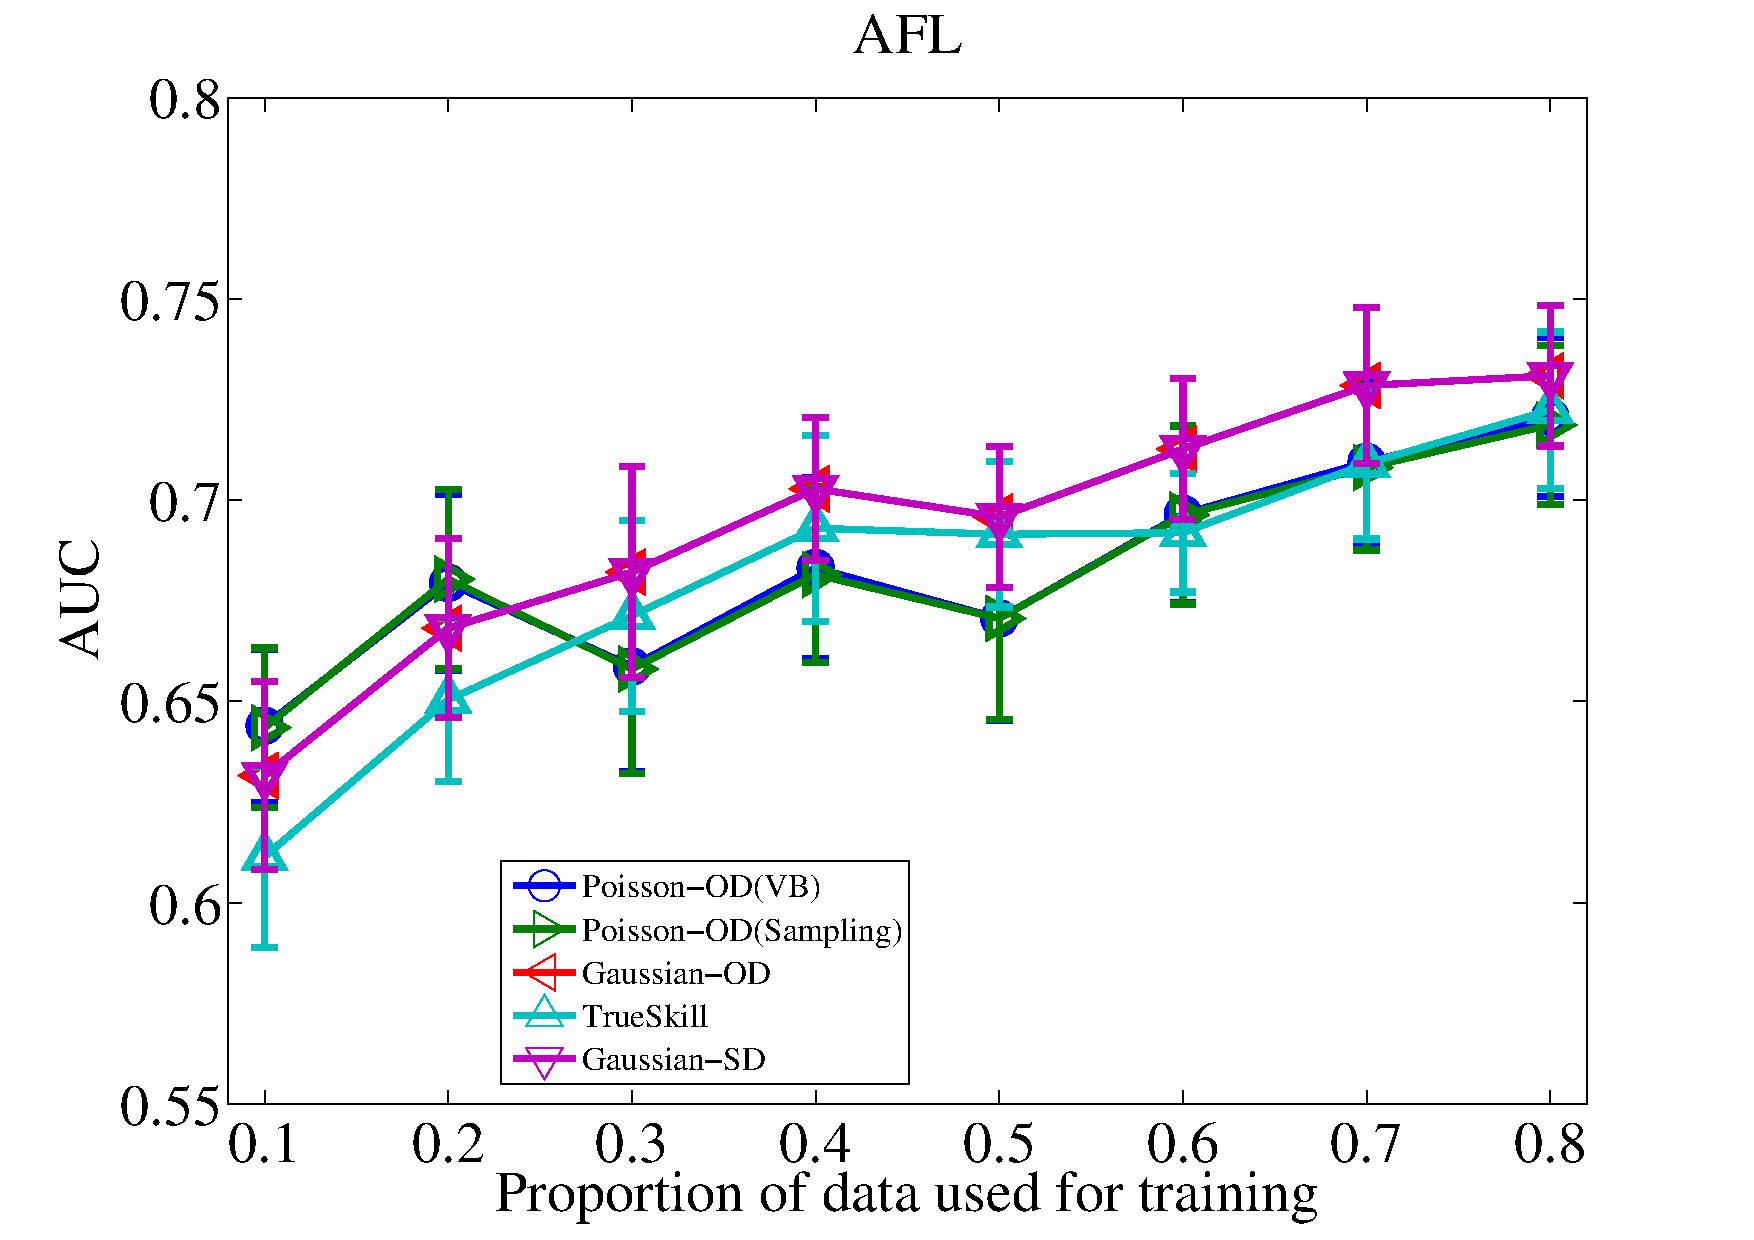
\epsfig{file=WLAccuracy_AFL, angle=0, height=3.6cm}
   \hspace{-0.725cm}
   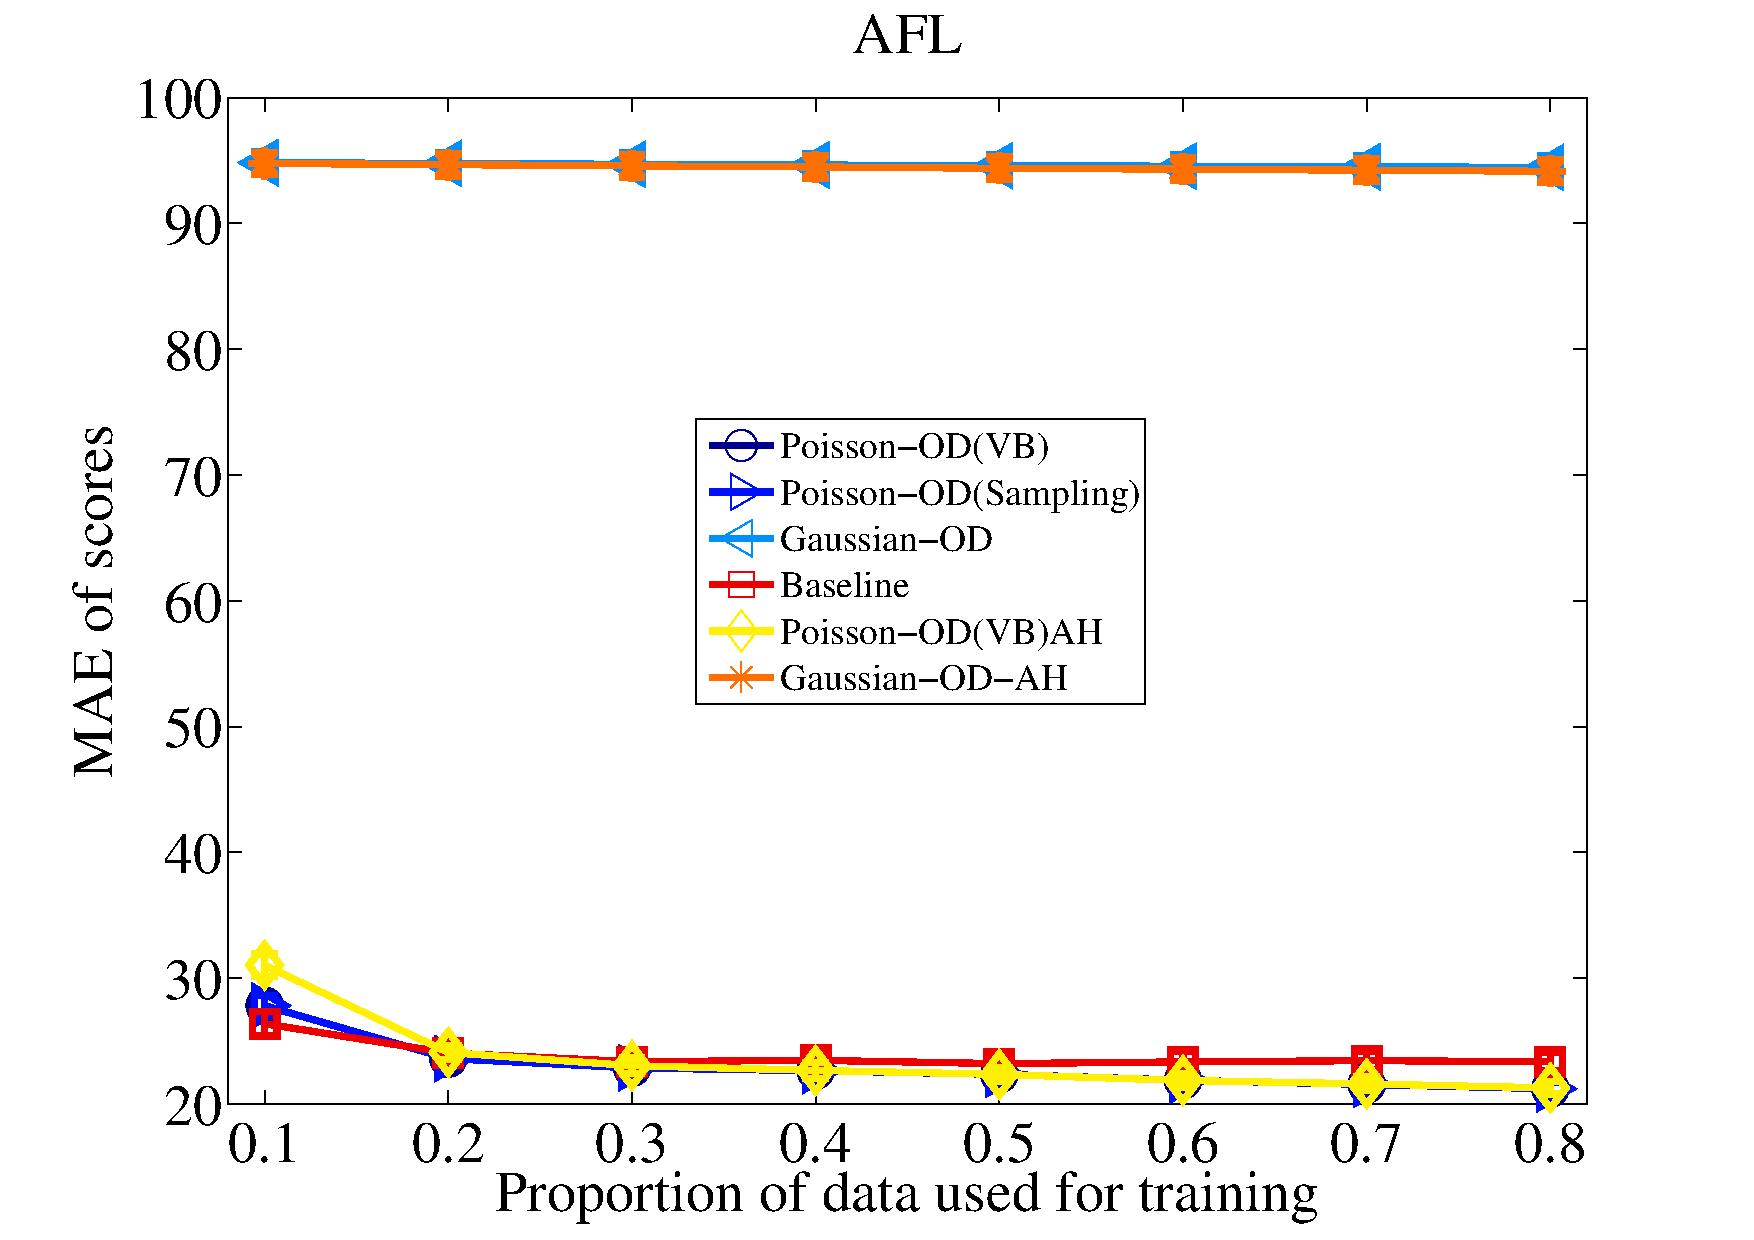
\epsfig{file=ScoreError_AFL, angle=0, height=3.6cm}
 }\\
\vspace{-0.3cm}
\caption{\small Results on the UK-PL, Halo, and AFL datasets evaluated
using information gain (left column), win/loss prediction accuracy in
term of the area of the curve (AUC) (middle column), and score
prediction error (right column).  Error bars indicate
95\% confidence intervals.}
\vspace{-0.3cm}
\label{fig:Results}
\end{figure*}
\end{center}
%%%%%%%%%%%%%%%%%%%%%%%%%%%%%%%%%%%%%%%%%%%%%%%%%%%%%%%%%%%%%%%%%

\subsubsection{Information Gain}
%\paragraph {Information Gain}

%Poisson-OD does not appear to provide accurate probability
%estimates in general -- we conjecture this could be due to biases
%introduced in the variational approximation scheme.
For relatively small amounts of training data (10\% -- 30\%), the
Gaussian models (OD and SD) statistically significantly outperform
TrueSkill and Poisson-OD in terms of win/loss probability accuracy.
On all data sets except AFL, the Gaussian models perform comparably to
TrueSkill for larger amounts of training data.  Gaussian-OD
statistically significantly outperforms Gaussian-SD for Halo 2,
indicating that separate offence/defence modeling helps.

%These results indicate that (a) score information can be very
%useful for making predictions when training data is limited;
%(b) separate offence/defence modeling seem to help Poisson-OD and Gaussian-OD
%outperform Gaussian-SD on Halo, and (c)
%the Poisson-OD model seems to predict more extreme probabilities, which
%can hurt it when its predictions are wrong.

\subsubsection{Win/no-Win Prediction Accuracy }
%\paragraph{Win/Loss Prediction Accuracy}

In terms of win/no-win prediction accuracy,
%Poisson-OD again does not
%generally perform as well as the other models -- we again conjecture
%this may be due to biases introduced in the variational approximation
%scheme.
the Gaussian-OD model generally
provides the best average AUC, followed by Gaussian-SD, then
TrueSkill (with the exception of cases for Halo 2 with more than 40\%
training data where TrueSkill performs best), then Poisson-oD.
Again, we see that
the separate offence/defence skill modeling of Gaussian-OD gives
it a performance edge over the combined skill model of Gaussian-SD.


%We check the statistics of the match outcomes
%(Table~\ref{table:datasetStatistics}),
%and observe that the average
%scores for the UK-PL, Halo, and AFL datasets are 1.3, 42.7, and 95.4,
%respectively.  From this, we might infer the Poisson-OD model predicts better
%when the average scores for a dataset are relatively larger numbers;
%here it seems the exponential term used in the Poisson model can help
%amplify small performance differences to explain high scores, leading
%to more stable skill modeling in high-scoring games.

\subsubsection{Score Prediction Errors}
%\paragraph{Score Prediction Errors}

%For the Gaussian-SD model, we note that the average relative score
%difference error is close 1 indicating the predicted difference is
%probably close to 0 with it being on the correct side of 0 as more
%training data is used.
%The Gaussian-OD model predicts more accurate scores on the UK-PL and
%Halo datasets, and Poisson-OD is more accurate for the AFL dataset.
%This can be explained by a simple skill analysis --- the learned
%skills on the UK-PL dataset tend to show a larger variance (for all
%models), whereas the learned skills on the AFL dataset show little
%variance (for all models except Gaussian-SD).  To confirm our
%previous hypothesis, the use of an exponentiated scoring rate in the
%Poisson model allows it to amplify small performance differences in
%the learned AFL skills to make more accurate score predictions on AFL
%data.  This amplification appears to hurt the Poisson-OD model on the
%relative low-scoring UK-PL dataset.

As shown in the third column in Figure~\ref{fig:Results}, Gaussian-OD
predicts more accurate scores on the UK-PL and Halo datasets, while
Poisson-OD is more accurate for the AFL dataset. This can be explained
by a simple skill analysis --- the learned skills on the UK-PL dataset
tend to show a larger variance (for all models), whereas the learned
skills on the AFL dataset show little variance (for all models except
Gaussian-SD). Thus, the use of an exponentiated scoring rate in the
Poisson-OD model would seem to amplify these small performance
differences in learned AFL skills to make more accurate score
predictions on AFL data.  This amplification appears to hurt the
Poisson-OD model on the lower-scoring UK-PL and Halo dataset (the mean
score for the AFL data is 95.4 vs 42.7 and 1.3 respectively for the
Halo 2 and UK-PL data).

%For the results on the Halo dataset, it is interesting to note that the Gaussian-OD and
%Poisson-OD models slightly outperform the Gaussian-SD model. This can
%perhaps be explained by the strength of modeling offence/defence
%skills separately. Note that both the Gaussian-OD and Poisson-OD
%models propose to treat offence and defence skills separately,
%contrasted with the Gaussian-SD model that uses a single skill
%variable.

\COMMENT
By referring to the score
statistics in Table~\ref{table:datasetStatistics}, our {\it
hypothesis} is that {\it the Poisson model is appropriate for
predicting scores when the match outcomes are given as relatively
larger numbers, which can be explained by its exponentiated rate that
allows to amplify small skill differences to predict the correct rates
needed for high scoring games}. Likewise the Gaussian model without
the exponentiation performs better for low scoring games.

In order to verify the hypothesis, we show the estimated skills after
training on the AFL and UK-PL dataset in
Figure~\ref{fig:ResultsEstimatedSKills}. On the AFL data set, the
differences across the skills of different teams learnt from the
Poisson model and Gaussian-S are relatively small, which supports the
above hypothesis.

%%%%%%%%%%%%%%%%%%%%%%%%%%%%%%%%%%%%%%%%%%%%%%%%%%%%%%%%%%%%%%%%%
\begin{figure*}[t!]
 \centering
 \vspace{-3cm}
 \subfigure{
   \hspace{-0.5cm}
   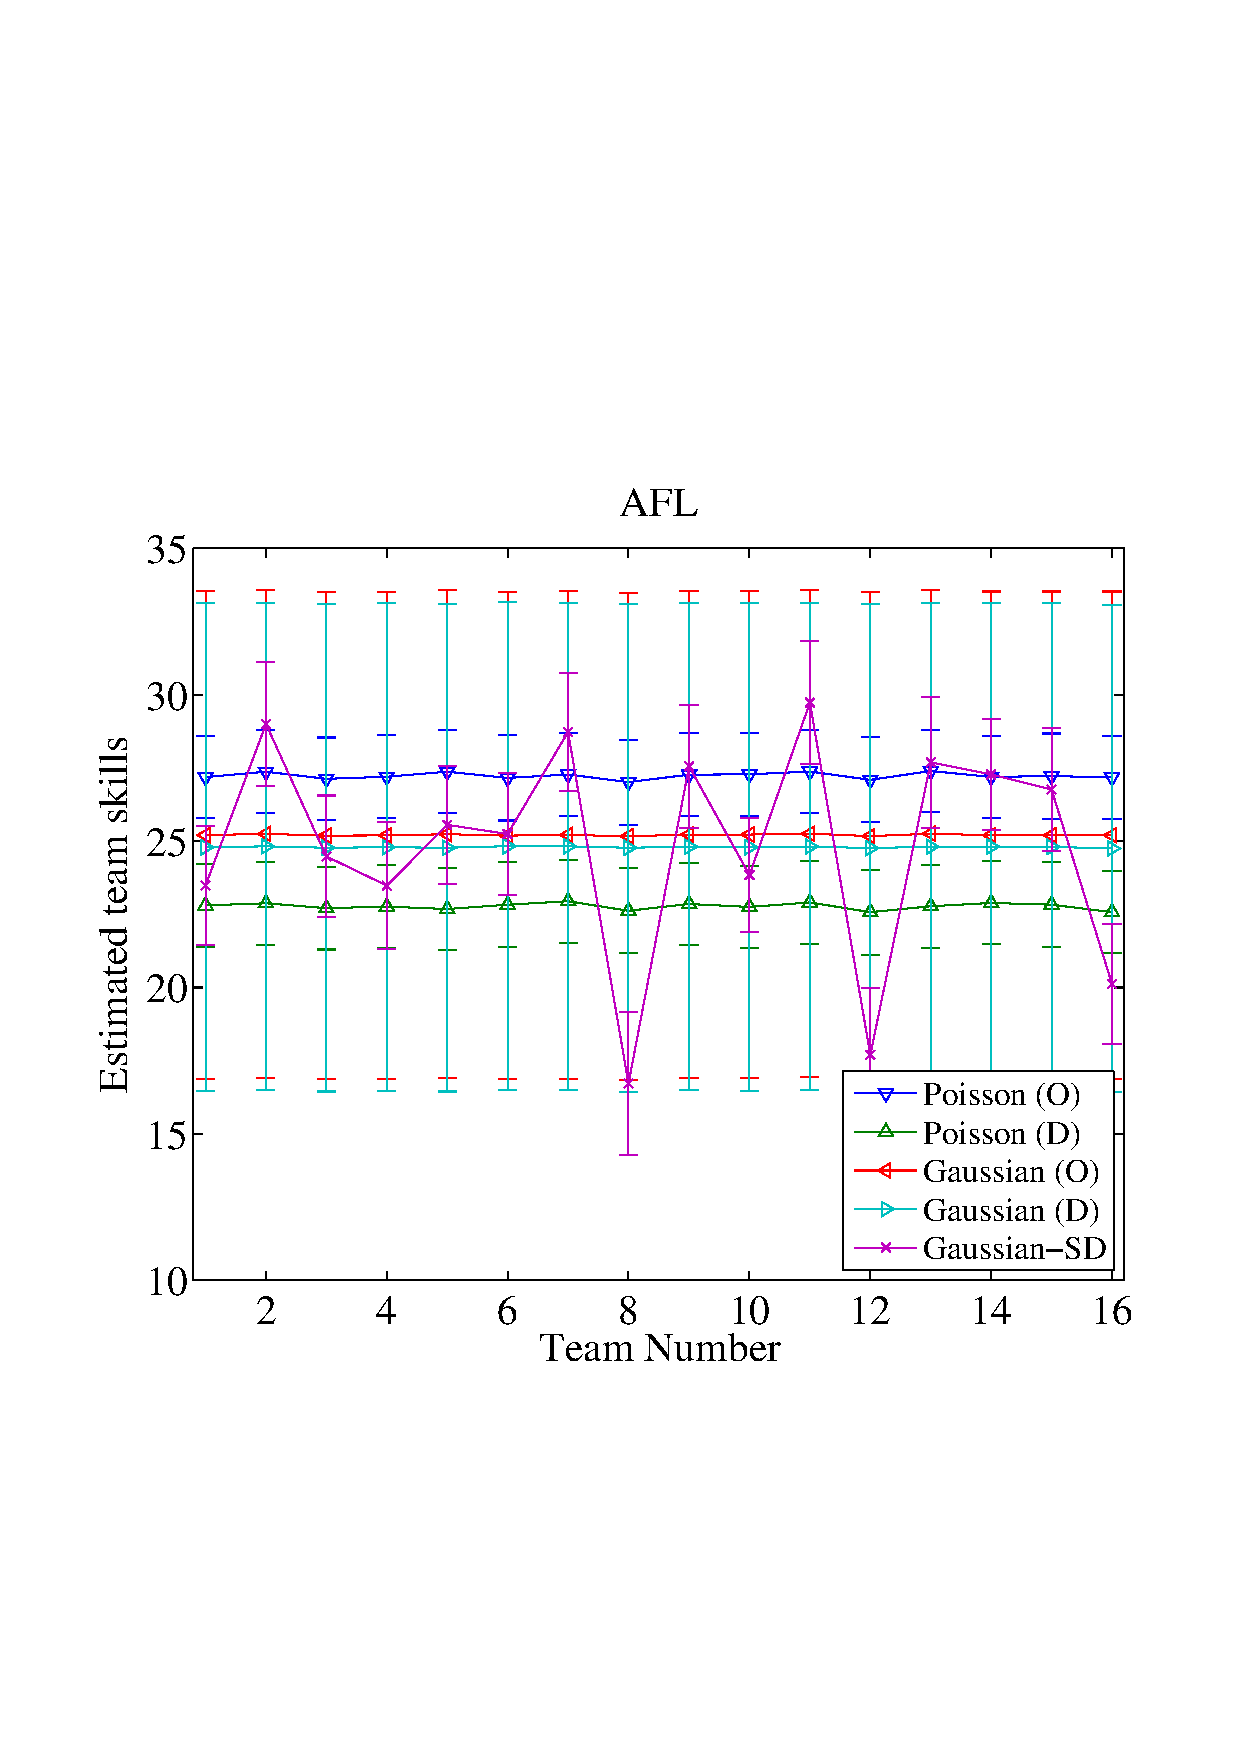
\epsfig{file=skillEstimation_AFL, angle=0, height=13cm}
  \hspace{-1.2cm}
   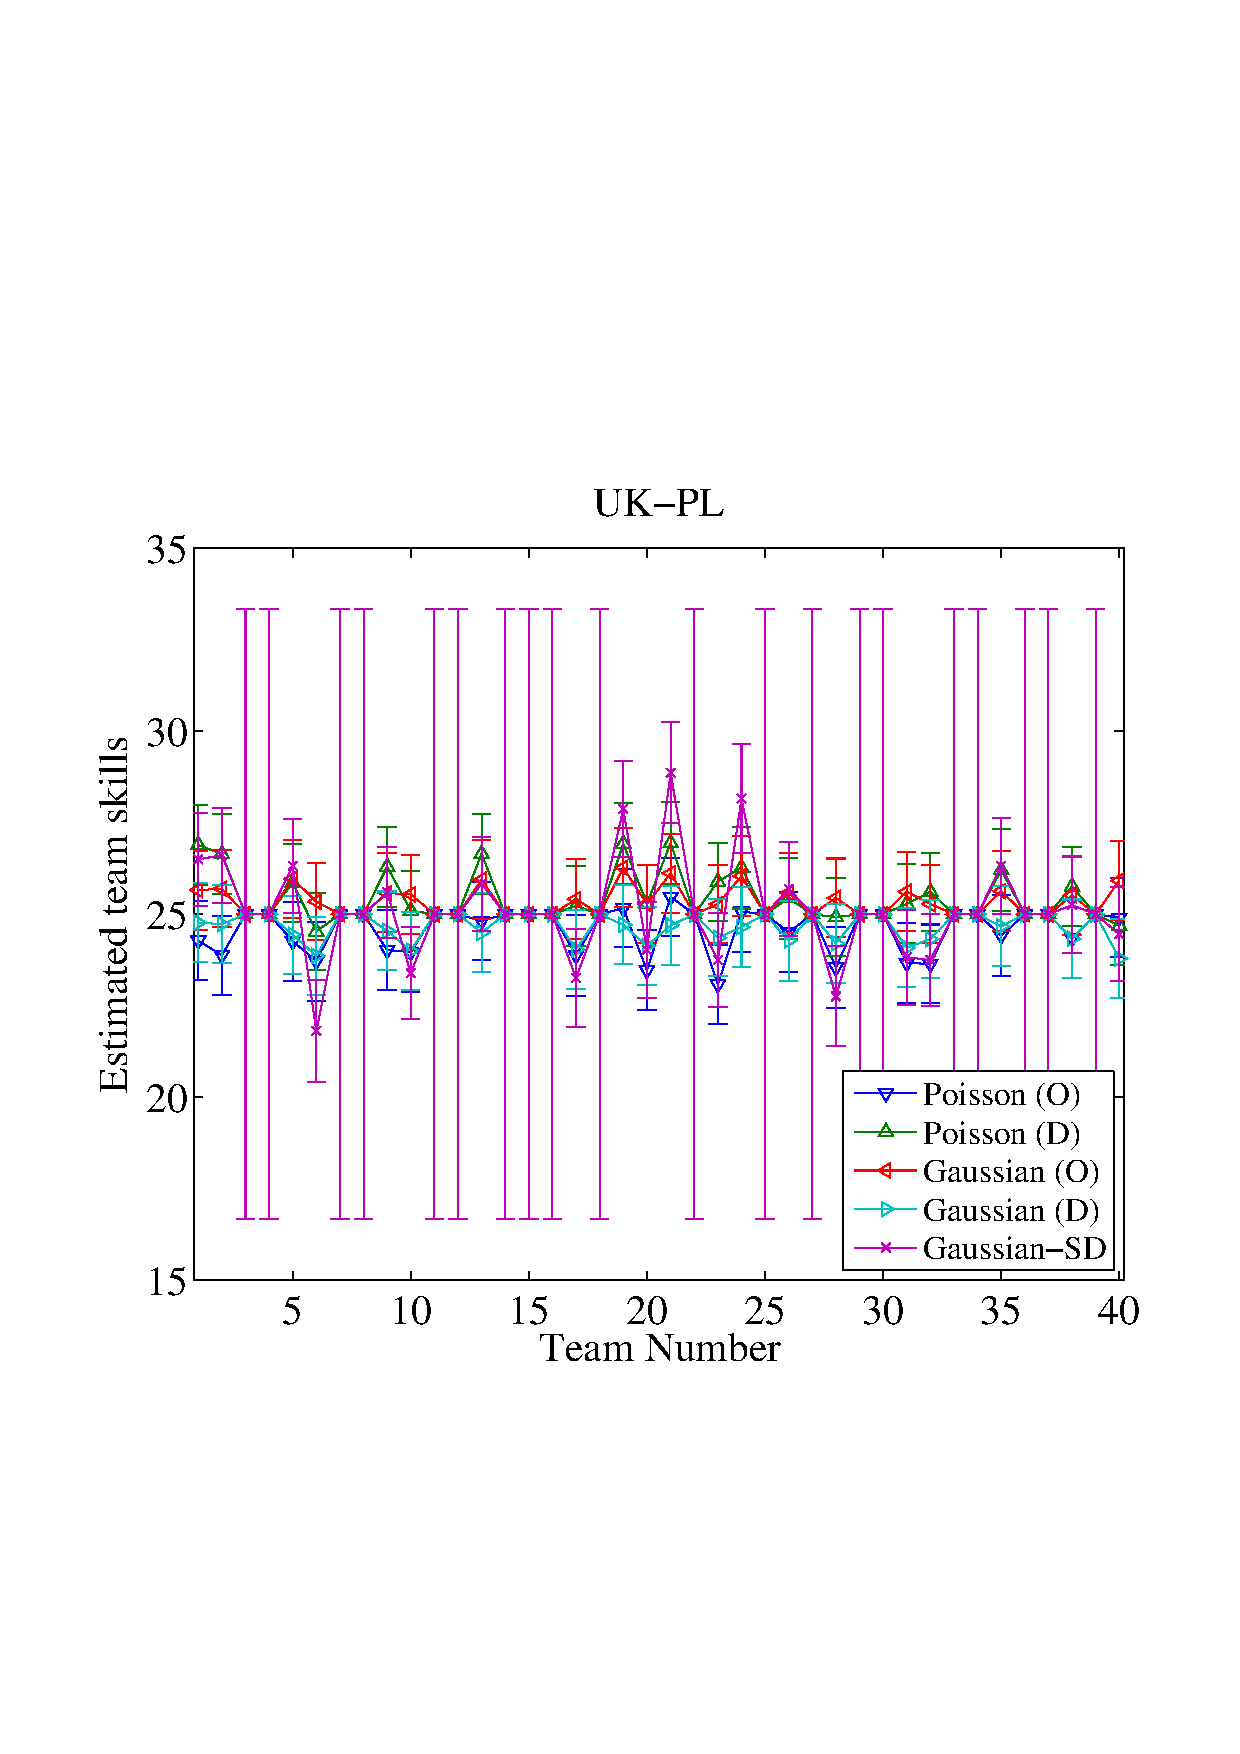
\epsfig{file=skillEstimation_UK, angle=0, height=13cm}
 }\\
 \vspace{-1.5cm}
\caption{Estimated skill levels of teams on the AFL (left) and UK-PL
  data (right) sets. Error bar indicates standard deviation.}
\label{fig:ResultsEstimatedSKills}
\end{figure*}
%%%%%%%%%%%%%%%%%%%%%%%%%%%%%%%%%%%%%%%%%%%%%%%%%%%%%%%%%%%%%%%%%

\ENDCOMMENT


\COMMENT
% JUST THREE NUMBERS, DON'T NEED A TABLE
%%%%%%%%%%%%%%%%%%%%%%%%%%%%%%%%%%%%%%%%%%%%%%%%%%%%%%%%%%%%%%%%%
\begin{table}
\caption{Score statistics for Halo, UK-PL, and AFL}
\begin{center}
\small
\begin{tabular}{|l|c|c|}
  \hline
  % after \\: \hline or \cline{col1-col2} \cline{col3-col4} ...
  Data set          & Mean and Standard Deviation\\
  \hline
  UK-PL             &  1.3023$\pm$1.2237 \\
  Halo 2 Beta     & 42.6929$\pm$3.0440 \\
  AFL                 &95.3784$\pm$27.8993 \\
  \hline
\end{tabular}
\label{table:datasetStatistics}
\end{center}
\end{table}
%%%%%%%%%%%%%%%%%%%%%%%%%%%%%%%%%%%%%%%%%%%%%%%%%%%%%%%%%%%%%%%%%
\ENDCOMMENT

% %TODO
% \begin{itemize}
%   \item Table: {\it testing on the last 10 percent data using models learnt from the first 90 percent data; Five by Three (algorithm by datasets);}
%   \item Performance vs. update \#: {\it testing on the last 10 percent data using models learnt from the first ${0.1, \cdots, 0.9}$ portion of the whole data set, for three data set -- 3 figures.}
%   \item Team rankings vs. o+d ranking (parallel lists in a table): {\it AFL and UK-PL give team ranking after each season. I will only evaluate on the team ranking for the last season. Two tables: one for AFL; the other for UK-PL.}
%   \item Score accuracy: {\it Poisson and Gaussian (S) -- score accuracy; Gaussian (SD) -- score difference accuracy;}
%   \item Bar graph predicted/actual win/lose draw: {\it three datasets, five algorithms, plot W/L/D frequency.}
%   \item Rel Info Gain???
% \end{itemize}
